% Drawing 142/02-1 -- folder 142, batch 02, archive page 23 (PDF page 24).
% Transcription: sphère vue en perspective ; sur l'équateur, trois points marqués (ronds pleins), chacun entouré d'un petit cercle portant deux sommets $R_i^{\omega}$, $R_i^{\omega'}$ ($i = 0, 1, \infty$), reliés par les arcs $a_i^{\omega}$, $a_i^{\omega'}$ ; les sommets voisins de deux points différents sont reliés par les flèches $b_0^{\omega}$, $b_1^{\omega}$ (lecture douteuse), $b_\infty^{\omega}$. Légende : $\mathrm{I}_J$.
% Kind: sphere with marked points, small circles and arrows. Method 2 (schematic redraw from the facsimile). Status: ok.
% Notes: Sphere outline and equator in pencil; the three marked points (big dots) on the equator, each in a small oriented circle with two vertices R_i^omega, R_i^omega'. Arrows b along the equator between the circles. The label of the right-hand b arrow is overinked; it is placed as the transcription reads it (b_1^omega, doubtful). The point near the north pole is drawn.
% Coordinates: 1 unit = 1 mm = 1/100 of the crop width (bbox in page fractions: [0.12, 0.09, 0.37, 0.24]).
% Redrawn by Claude (claude-opus-5-5), issue #73, 2026-11-07; not checked by a human; not compiled (no TeX in the session).
% Rights: reproduces part of the work -- behind RENDER_TRANSCRIPTS, never published by itself.
\documentclass[tikz,border=3pt]{standalone}
\usepackage{amsmath,amssymb}
\usetikzlibrary{patterns,arrows.meta}
\tikzset{pencil/.style={black!45}, struck/.style={black!35}, mark/.style={circle,draw,inner sep=1.3pt}, pt/.style={circle,fill,inner sep=0.9pt}, opt/.style={circle,draw,fill=white,inner sep=1.1pt}}
\begin{document}
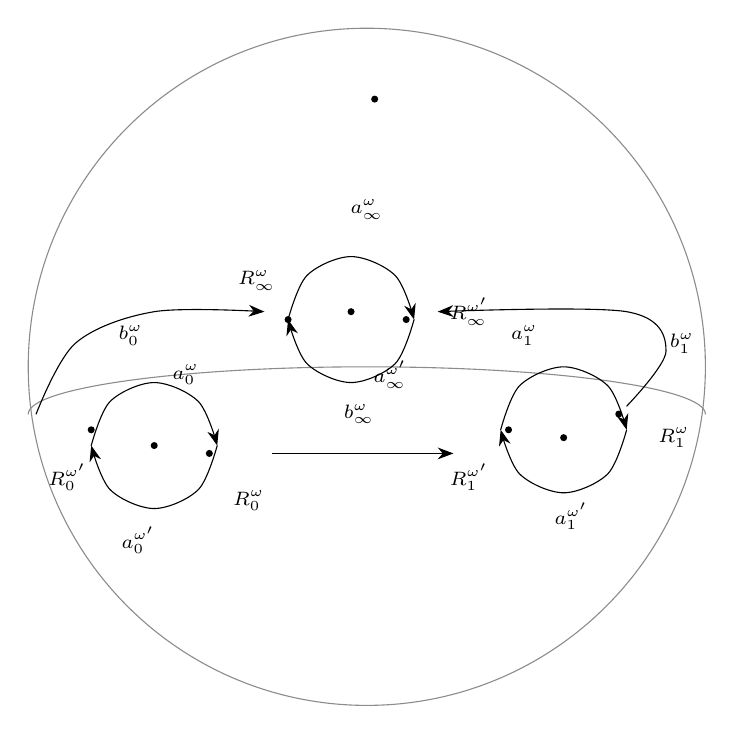
\begin{tikzpicture}[x=1mm,y=1mm,line cap=round,line join=round,font=\scriptsize]
\draw[pencil] (57,-50) circle[radius=43];
\draw[pencil] (100,-56) arc[start angle=0, end angle=180, x radius=43, y radius=6];
\node[pt] at (58,-16) {};
\node[pt] at (30,-60) {};
\node[pt] at (55,-43) {};
\node[pt] at (82,-59) {};
\draw[-{Stealth[length=2mm]}] plot[smooth, tension=0.55] coordinates {(22,-60) (24.4,-54.4) (30,-52) (35.6,-54.4) (38,-60)};
\draw[-{Stealth[length=2mm]}] plot[smooth, tension=0.55] coordinates {(38,-60) (35.6,-65.6) (30,-68) (24.4,-65.6) (22,-60)};
\draw[-{Stealth[length=2mm]}] plot[smooth, tension=0.55] coordinates {(47,-44) (49.4,-38.4) (55,-36) (60.6,-38.4) (63,-44)};
\draw[-{Stealth[length=2mm]}] plot[smooth, tension=0.55] coordinates {(63,-44) (60.6,-49.6) (55,-52) (49.4,-49.6) (47,-44)};
\draw[-{Stealth[length=2mm]}] plot[smooth, tension=0.55] coordinates {(74,-58) (76.4,-52.4) (82,-50) (87.6,-52.4) (90,-58)};
\draw[-{Stealth[length=2mm]}] plot[smooth, tension=0.55] coordinates {(90,-58) (87.6,-63.6) (82,-66) (76.4,-63.6) (74,-58)};
\node[pt] at (22,-58) {};
\node[pt] at (37,-61) {};
\node[pt] at (47,-44) {};
\node[pt] at (62,-44) {};
\node[pt] at (75,-58) {};
\node[pt] at (89,-56) {};
\draw[-{Stealth[length=2mm]}] plot[smooth, tension=0.55] coordinates {(15,-56) (20,-47) (30,-43) (44,-43)};
\draw[-{Stealth[length=2mm]}] (45,-61) -- (68,-61);
\draw[-{Stealth[length=2mm]}] plot[smooth, tension=0.55] coordinates {(90,-55) (95,-48) (90,-43) (66,-43)};
\node[inner sep=1pt] at (43,-39) {\scriptsize $R_\infty^{\omega}$};
\node[inner sep=1pt] at (70,-43) {\scriptsize $R_\infty^{\omega'}$};
\node[inner sep=1pt] at (19,-64) {\scriptsize $R_0^{\omega'}$};
\node[inner sep=1pt] at (42,-67) {\scriptsize $R_0^{\omega}$};
\node[inner sep=1pt] at (70,-64) {\scriptsize $R_1^{\omega'}$};
\node[inner sep=1pt] at (96,-59) {\scriptsize $R_1^{\omega}$};
\node[inner sep=1pt] at (57,-30) {\scriptsize $a_\infty^{\omega}$};
\node[inner sep=1pt] at (60,-51) {\scriptsize $a_\infty^{\omega'}$};
\node[inner sep=1pt] at (34,-51) {\scriptsize $a_0^{\omega}$};
\node[inner sep=1pt] at (28,-72) {\scriptsize $a_0^{\omega'}$};
\node[inner sep=1pt] at (77,-46) {\scriptsize $a_1^{\omega}$};
\node[inner sep=1pt] at (83,-69) {\scriptsize $a_1^{\omega'}$};
\node[inner sep=1pt] at (27,-46) {\scriptsize $b_0^{\omega}$};
\node[inner sep=1pt] at (56,-56) {\scriptsize $b_\infty^{\omega}$};
\node[inner sep=1pt] at (97,-47) {\scriptsize $b_1^{\omega}$};
\end{tikzpicture}
\end{document}
